\tikzstyle{block} = [rectangle, draw, fill=blue!20, text centered]
\begin{center}
	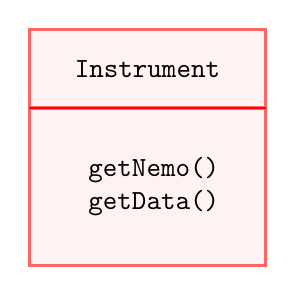
\begin{tikzpicture}
		%\node [block] (madre) {Instrument};
		%\node [block, below of=madre] {InstrumentRV};
		% Cajas
		\filldraw[color=red!60, fill=red!5, very thick] (0,0) rectangle (3,2);
		\filldraw[color=red!60, fill=red!5, very thick] (0,2) rectangle (3,3);
		\draw[thick, red, -] (0,2) -- (3,2);
		% Tamaños de las cajas
		\node[] at (1.5,2.5) {\texttt{Instrument}};
		\node[text width=1.5cm,text centered] at (1.5,1) {
			\texttt{getNemo()}
			\texttt{getData()}
		};
		% Aristas
		
		%\draw[thick,red,-] (1.5,0) -- (4.5,0) ;
		
		% Cajas
		%\node [draw, thick, shape=rectangle, minimum width=3cm, minimum height=3cm, anchor=center, color=blue] at (0,0) {};
		%\node [draw, thick, shape=rectangle, minimum width=3cm, minimum height=3cm, anchor=center, color=blue] at (6,0) {};
	\end{tikzpicture}
\end{center}